\section{Обсуждение результатов и оценка}
Мы обсудим некоторые детали реализации, представим результаты и проведем оценку нашего алгоритма в сравнении с предыдущими работами, а также проведем исследование по удалению компонентов.

\subsection{Реализация}
\label{sec:impl}
Мы реализовали наш метод на Python с использованием фреймворка PyTorch и написали пользовательские CUDA-ядра для растеризации, которые являются расширенными версиями предыдущих методов~\cite{kopanas21}, и используем библиотеку NVIDIA CUB для быстрой сортировки Radix sort~\cite{merrill2010revisiting}.
Также мы создали интерактивный просмотрщик, используя открытый исходный код SIBR~\cite{sibr2020}, который используется для интерактивного просмотра. \ADDITION{Мы использовали эту реализацию для измерения достигнутой частоты кадров}.
Исходный код и все наши данные доступны по адресу: \textcolor{blue}{\url{https://repo-sam.inria.fr/fungraph/3d-gaussian-splatting/}} 

\paragraph{Детали оптимизации}
Для стабильности мы «разогреваем» вычисления в более низком разрешении.
В частности, мы начинаем оптимизацию, используя изображения с разрешением в 4 раза ниже и увеличиваем их дважды после 250 и 500 итераций.
Оптимизация коэффициентов SH чувствительна к недостатку угловой информации. Для типичных «NeRF-like»
захватов, где центральный объект наблюдается с помощью фотографий, сделанных по всему полушарию вокруг него, оптимизация работает хорошо. Однако, если захват имеет пропущенные угловые области (например, при захвате угла сцены или выполнении «внутрь-наружу»~\cite{HRDB16} захвата), полностью некорректные значения для нулевого компонента SH (т.е., базового или диффузного цвета) могут быть получены в результате оптимизации.
Чтобы преодолеть эту проблему, мы начинаем с оптимизации только нулевого компонента, а затем вводим одну полосу SH после каждых 1000 итераций, пока все 4 полосы SH не будут представлены. %

\begin{table*}[!h]
    \caption{Оценка PSNR для тестовых прогонов. \ADDITION{Для этого эксперимента мы вручную понизили разрешение высококачественных версий входных изображений каждой сцены до установленного разрешения рендеринга наших других экспериментов. Это снижает случайные артефакты (например, из-за сжатия JPEG в предварительно уменьшенных входных данных Mip-NeRF360).}}
    \centering
    \begin{tabular}{l|ccc|ccc|cc}
        ~ & Truck-5K & Garden-5K & Bicycle-5K & Truck-30K & Garden-30K & Bicycle-30K & Average-5K & Average-30K \\ \hline
        Limited-BW  & 14.66 & 22.07 & 20.77 & 13.84 & 22.88 & 20.87 & 19.16 & 19.19 \\
        Random Init & 16.75 & 20.90 & 19.86 & 18.02 & 22.19 & 21.05 & 19.17 & 20.42 \\ 
        No-Split    & 18.31 & 23.98 & 22.21 & 20.59 & 26.11 & 25.02 & 21.50 & 23.90 \\ 
        No-SH       & \cellcolor{yellow!40}22.36 & 25.22 & \cellcolor{orange!40}22.88 & \cellcolor{yellow!40}24.39 & 26.59 & \cellcolor{yellow!40}25.08 & \cellcolor{yellow!40}23.48 & \cellcolor{yellow!40}25.35 \\ 
        No-Clone    & 22.29 & \cellcolor{orange!40}25.61 & 22.15 & \cellcolor{red!40}24.82 & \cellcolor{orange!40}27.47 & \cellcolor{orange!40}25.46 & 23.35 & \cellcolor{orange!40}25.91 \\  
        Isotropic   & \cellcolor{orange!40}22.40 & \cellcolor{yellow!40}25.49 & \cellcolor{yellow!40}22.81 & 23.89 & \cellcolor{yellow!40}27.00 & 24.81 & \cellcolor{orange!40}23.56 & 25.23 \\  
        Full        & \cellcolor{red!40}22.71 & \cellcolor{red!40}25.82 & \cellcolor{red!40}23.18 & \cellcolor{orange!40}24.81 &\cellcolor{red!40} 27.70 & \cellcolor{red!40}25.65 & \cellcolor{red!40}23.90 & \cellcolor{red!40}26.05 \\  
    \end{tabular}
    \label{tab:ablation_table}
\end{table*}

\subsection{Результаты и оценка}
\paragraph{Результаты.}
Мы протестировали наш алгоритм на общем количестве \CORRECTION{11}{13} реальных сцен, взятых из ранее опубликованных наборов данных и синтетического набора данных Blender ~\cite{mildenhall2020nerf}. 
В частности, мы протестировали наш подход на полном наборе сцен, представленных в Mip-Nerf360~\cite{barron2022mipnerf360}, который является текущим уровнем качества рендеринга NeRF, двух сценах из набора данных Tanks\&Temples \shortcite{knapitsch2017tanks} и двух сценах, предоставленных Hedman et al.~\cite{hedman2018deep}. 
Сцены, которые мы выбрали, имеют очень разные стили захвата, и охватывают как ограниченные внутренние сцены, так и большие неограниченные внешние среды.
\CORRECTION{Мы используем одинаковые значения параметров для всех наших запусков, за исключением скорости обучения для ковариации: для всех сцен она составляет 0.001, за исключением \textsc{Train}, \textsc{DrJohnson} и \textsc{Playroom} (см. Рис.~\mbox{\ref{fig:comparisons}}), где она делится на три, поскольку стиль захвата намного менее структурирован.}{Мы используем ту же конфигурацию гиперпараметров для всех экспериментов в нашей оценке.} Все результаты указаны для работы на GPU A6000\ADDITION{, за исключением метода Mip-NeRF360 (см. ниже)}.
В дополнительных материалах мы показываем видео пути рендеринга для выбора сцен, содержащих виды, далекие от входных фотографий.

\paragraph{Реальные сцены.}
В плане качества текущий уровень развития — это Mip-Nerf360~\cite{barron2021mipnerf}. Мы сравниваемся с этим методом как с качественным эталоном. Мы также сравниваемся с двумя самыми последними быстрыми методами NeRF: InstantNGP~\cite{mueller2022instant} и Plenoxels~\cite{plenoxels}.
Мы используем разделение train/test для наборов данных, используя методологию, предложенную Mip-NeRF360, беря каждую 8-ю фотографию для теста, для последовательных и значимых сравнений для генерации метрик ошибок, используя стандартные метрики PSNR, L-PIPS и SSIM, наиболее часто используемые в литературе; пожалуйста, см. \CORRECTION{Таб.}{Таблица}~\ref{tab:comparisons}. \CORRECTION{Обратите внимание, что мы запустили улучшенную версию кода Mip-NeRF360, которая дает немного лучшие числа, чем в оригинальной публикации.}{Все числа в таблице взяты из наших собственных запусков кода авторов для всех предыдущих методов, за исключением тех, что относятся к Mip-NeRF360 на их наборе данных, где мы скопировали числа из оригинальной публикации, чтобы избежать путаницы о текущем уровне развития. Для изображений в наших
фигурах мы использовали наш собственный запуск Mip-NeRF360: числа для этих запусков находятся в Приложении~\ref{sec:appd}.}
Мы также показываем среднее время обучения, скорость рендеринга и объем памяти, используемый для хранения оптимизированных параметров. Мы сообщаем результаты для базовой конфигурации InstantNGP (Base), которая работает в течение 35K итераций, а также немного большей сети, предложенной авторами (Big), и двух конфигураций, 7K и 30K итераций для нашего метода. 
Мы показываем разницу в визуальном качестве для наших двух конфигураций на Рис.~\ref{fig:5vs40min}. Во многих случаях качество после 7K итераций уже довольно хорошее.
Время обучения различается в зависимости от наборов данных, и мы сообщаем их отдельно. Обратите внимание, что разрешение изображений также различается в зависимости от наборов данных.
В \CORRECTION{дополнительных материалах}{проектном сайте} мы предоставляем все рендеры тестовых видов, которые мы использовали для вычисления статистики для всех методов (наших и предыдущих работ) на \CORRECTION{\textsc{bicycle}, \textsc{Truck} и \textsc{Playroom}}{все сцены.} Обратите внимание, что мы сохранили исходное входное разрешение для всех рендеров.
Таблица показывает, что наша полностью сходившаяся модель достигает качества наравне и иногда немного лучше, чем у лидирующего метода Mip-NeRF360; обратите внимание, что на том же оборудовании их среднее время обучения составило 48 часов\footnote{Мы обучали Mip-NeRF360 на узле с 4 GPU A100 в течение 12 часов, что эквивалентно 48 часам на одном GPU. Обратите внимание, что A100 быстрее, чем GPU A6000.}, по сравнению с нашими 35-45 минутами, а их время рендеринга составляет 10 секунд/кадр. Мы достигаем сравнимого качества с InstantNGP и Plenoxels после 5-10 минут обучения, но дополнительное время обучения позволяет нам достичь уровня современного развития, чего нельзя сказать о других быстрых методах. Для Tanks \& Temples мы достигаем аналогичного качества как базовый InstantNGP при аналогичном времени обучения ($\sim$\CORRECTION{8}{7} минут в нашем случае).
Мы также показываем визуальные результаты этого сравнения для тестового вида для нашего метода и предыдущих методов рендеринга, выбранных для сравнения, на Рис.~\ref{fig:comparisons}; результаты нашего метода после 30K итераций обучения. Мы видим, что в некоторых случаях даже Mip-NeRF360 имеет оставшиеся артефакты, которых избегает наш метод (например, размытость в растительности — в \textsc{Bicycle, Stump} — или на стенах в \textsc{Room}).
В дополнительном видео и на веб-странице мы предоставляем сравнения путей с расстояния. Наш метод сохраняет визуальные детали хорошо покрытых областей даже с дальнего расстояния, чего не всегда можно добиться другими методами.

\paragraph{Синтетические ограниченные сцены}
Помимо реалистичных сцен, мы также оцениваем наш подход на синтетическом наборе данных \emph{Blender} \cite{mildenhall2020nerf}. Сцены в вопросе предоставляют исчерпывающий набор видов, ограничены в размере и предоставляют точные параметры камеры. В таких сценариях мы можем достичь результатов уровня современного состояния даже с произвольной инициализацией: мы начинаем обучение с 100K равномерно случайных Гауссиан внутри объема, охватывающего границы сцены. Наш подход быстро и автоматически сокращает их до примерно 6--10K значимых Гауссиан. Конечный размер обученной модели после 30K итераций достигает около 200--500K Гауссиан на сцену. Мы сообщаем и сравниваем наши достигнутые значения PSNR с предыдущими методами в \CORRECTION{Таб.}{Таблица}~\ref{tab:results_synthetic} с использованием белого фона для совместимости. Примеры можно увидеть на Рис.~\ref{fig:ablation-aniso} (второе изображение слева) и в дополнительных материалах. \ADDITION{Обученные синтетические сцены рендерятся со скоростью 180--300 FPS.}

\paragraph{Компактность}
В сравнении с предыдущими явными представлениями сцен, анизотропные Гауссианы, используемые в нашей оптимизации, способны моделировать сложные формы с меньшим количеством параметров.
Мы демонстрируем это, оценивая наш подход против высоко компактных, основанных на точках моделей, полученных \cite{zhang2022}.
Мы начинаем с их начального облака точек, которое получено путем пространственного вырезания с масками переднего плана %
и оптимизируем, пока не достигнем равенства с их заявленными значениями PSNR. Обычно это происходит в течение 2--4 минут. Мы превышаем их заявленные метрики, используя примерно четверть их количества точек, что приводит к среднему размеру модели 3.8 МБ, по сравнению с их 9 МБ. Мы отмечаем, что для этого эксперимента мы использовали только две степени наших сферических гармоник, аналогично их подходу.

\subsection{Исследования по удалению компонентов}
\label{sec:ablations}
Мы выделили различные вклады и алгоритмические решения, которые мы приняли, и создали серию экспериментов для измерения их влияния. В частности, мы тестируем следующие аспекты нашего алгоритма: инициализация из SfM, наши стратегии уплотнения, анизотропная ковариация, тот факт, что мы позволяем неограниченному количеству сплатов иметь градиенты
и использование сферических гармоник.
Количественное влияние каждого выбора суммировано в \CORRECTION{Таб.}{Таблица}~\ref{tab:ablation_table}.

\begin{figure}[!h]
    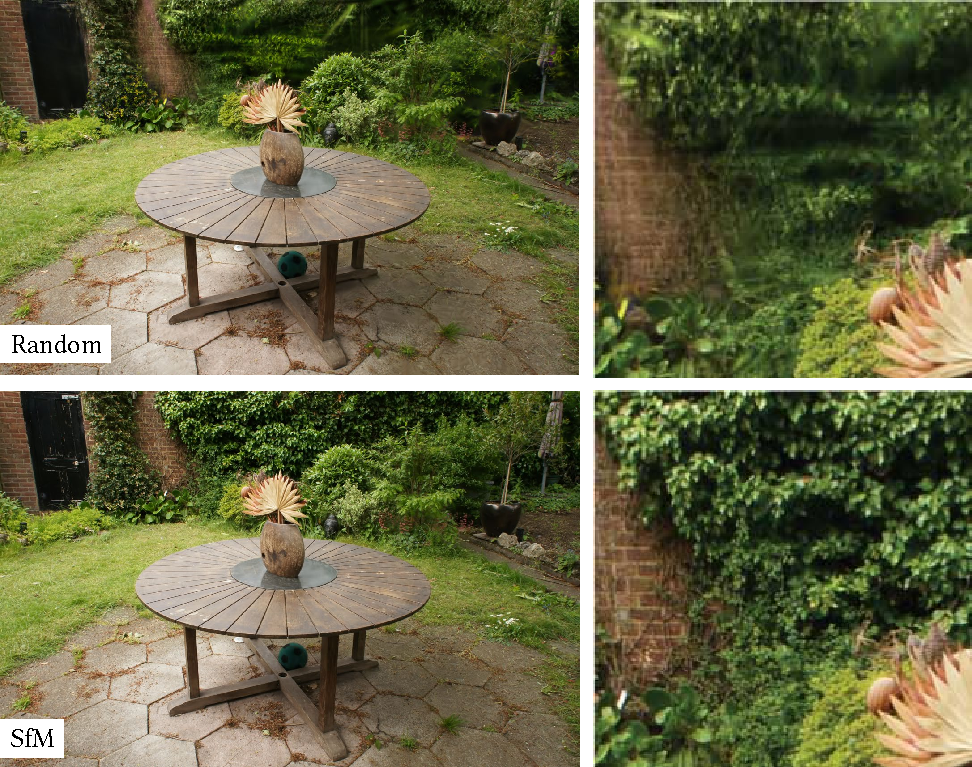
\includegraphics[width=\linewidth]{figures/ablations/random_vs_sfm2.pdf}
    \caption{
        \label{fig:random}
        Инициализация с точками SfM помогает. Выше: инициализация с случайным облаком точек. Ниже: инициализация с использованием точек SfM.
    }
\end{figure}

\paragraph{Инициализация из SfM}
Мы также оцениваем важность инициализации 3D Гауссиан из облака точек SfM.
Для этого исследования мы равномерно выбираем куб с размером, равным трем размерам ограничивающего прямоугольника входных камер. Мы наблюдаем, что наш метод работает относительно хорошо, избегая полного провала даже без точек SfM. Вместо этого он ухудшается в основном на заднем плане, см. Рис.~\ref{fig:random}. Также в областях, плохо покрытых обучающими видами, метод случайной инициализации кажется более подверженным наличию "плавающих" точек, которые не могут быть удалены оптимизацией. С другой стороны, синтетический набор данных NeRF не проявляет такого поведения, потому что у него нет заднего плана и он хорошо ограничен входными камерами (см. обсуждение выше).

\begin{figure}[!h]
    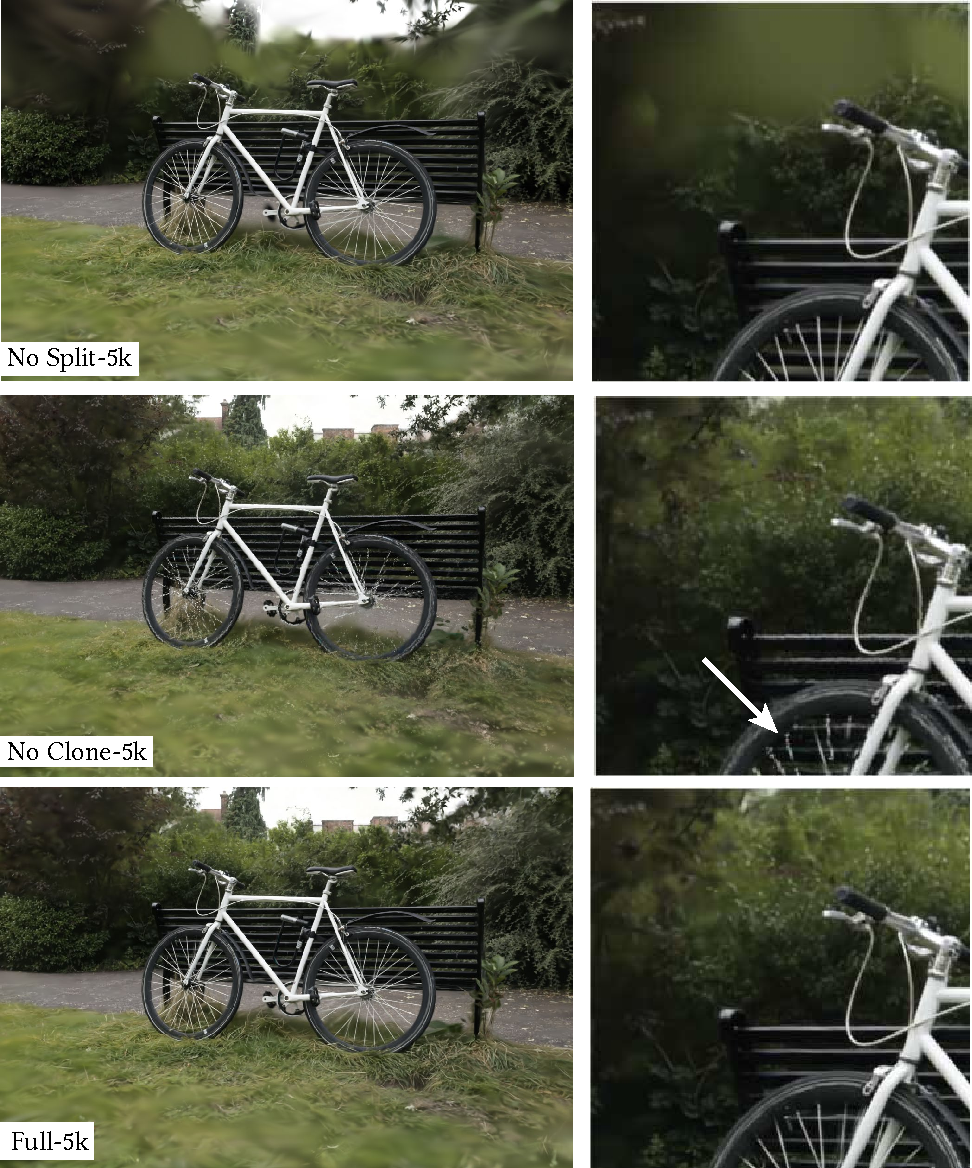
\includegraphics[width=\linewidth]{figures/ablations/densification.pdf}
    \caption{
        \label{fig:densification_ablate}
        Исследование стратегии уплотнения для двух случаев "клонирование" и "разделение" (Раздел~\ref{sec:opt-dens}).
    }
\end{figure}

\paragraph{Уплотнение.}
Мы далее оцениваем наши два метода уплотнения, а именно стратегию клонирования и разделения, описанные в Разделе~\ref{sec:opt-dens}. Мы отключаем каждый метод по отдельности и оптимизируем, используя остальную часть метода без изменений. Результаты показывают, что разделение больших Гауссиан важно для обеспечения хорошей реконструкции заднего плана, как видно на Рис.~\ref{fig:densification_ablate}, тогда как клонирование маленьких Гауссиан вместо их разделения позволяет достичь лучшей и более быстрой сходимости, особенно когда в сцене появляются тонкие структуры.

\begin{figure}[!h]
    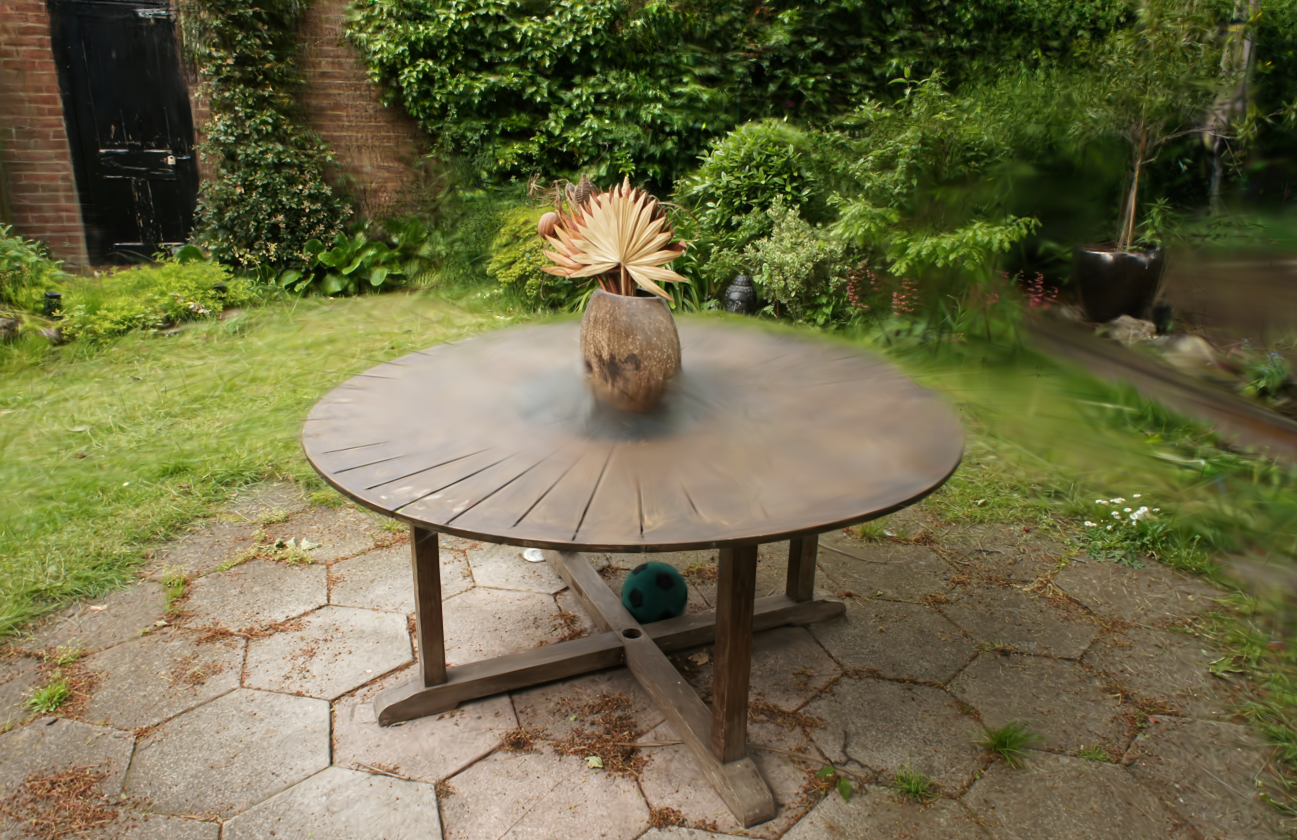
\includegraphics[width=.49\linewidth]{figures/ablations/images/30k/garden/limitedBW.png}
    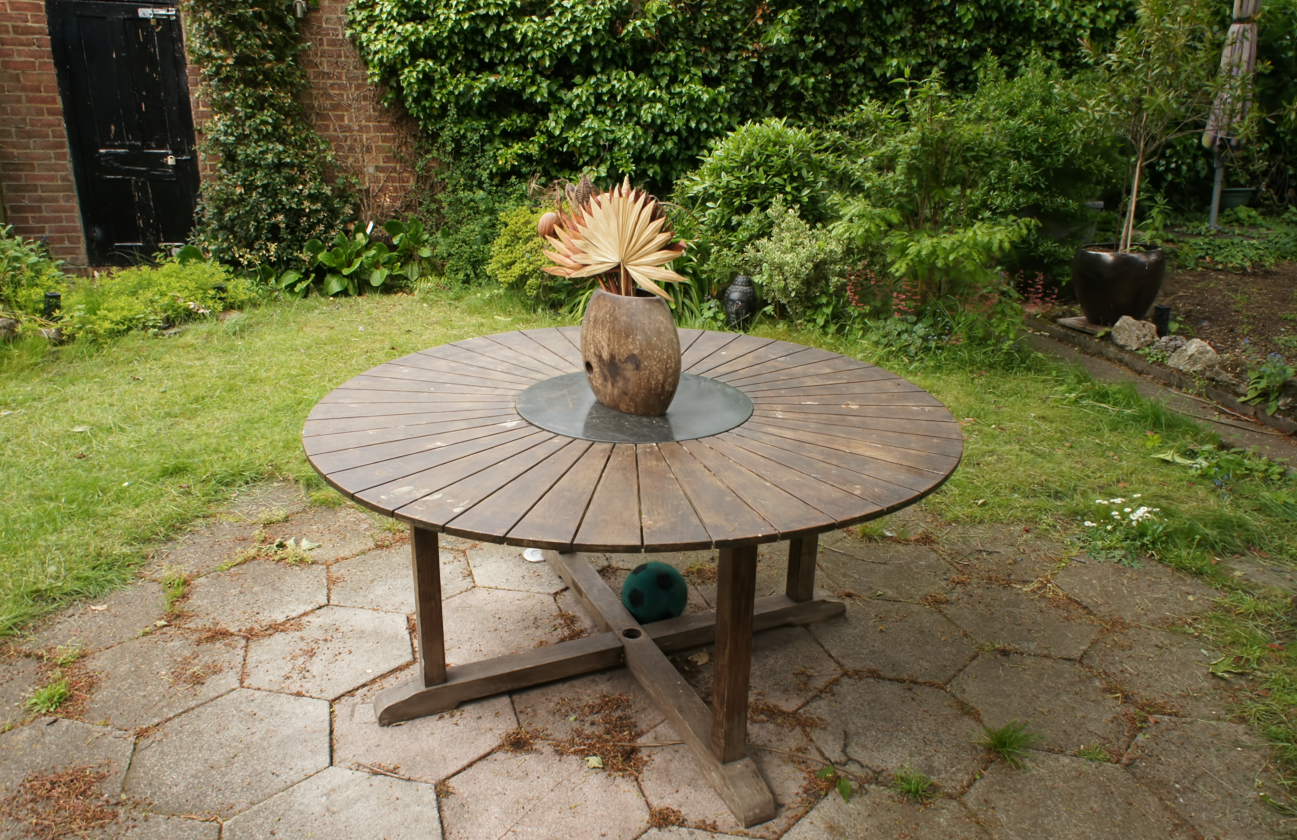
\includegraphics[width=.49\linewidth]{figures/ablations/images/30k/garden/full.png}
    \caption{
        Если мы ограничим количество точек, получающих градиенты, эффект на визуальное качество будет значительным.
        Слева: лимит в 10 Гауссиан, получающих градиенты. Справа: наш полный метод.
        \label{fig:gradients}
    }
\end{figure}

\paragraph{Неограниченная глубина сложности сплатов с градиентами.}
Мы оцениваем, даст ли пропуск вычисления градиентов после $N$ передних точек нам скорость без ущерба для качества, как предложено в Pulsar~\cite{Lassner_2021_CVPR}. В этом тесте мы выбираем N=10, что в два раза больше значения по умолчанию в Pulsar, но это привело к нестабильной оптимизации из-за серьезного приближения в вычислении градиентов. Для сцены \textsc{Truck} качество ухудшилось на 11 дБ в PSNR (см. \CORRECTION{Таб.}{Таблица}~\ref{tab:ablation_table}, Limited-BW), и визуальный результат показан на Рис.~\ref{fig:gradients} для \textsc{Garden}.

\paragraph{Анизотропная ковариация.}
Важным алгоритмическим выбором в нашем методе является оптимизация полной матрицы ковариации для 3D Гауссиан. Чтобы продемонстрировать влияние этого выбора, мы проводим исследование, где удаляем анизотропию, оптимизируя одно скалярное значение, которое управляет радиусом 3D Гауссиана по всем трем осям. Результаты этой оптимизации представлены визуально на Рис.~\ref{fig:ablation-aniso}. Мы наблюдаем, что анизотропия значительно улучшает способность 3D Гауссиан выравниваться с поверхностями, что, в свою очередь, позволяет достичь гораздо более высокого качества рендеринга, сохраняя то же количество точек.

\begin{figure*}[!h]
    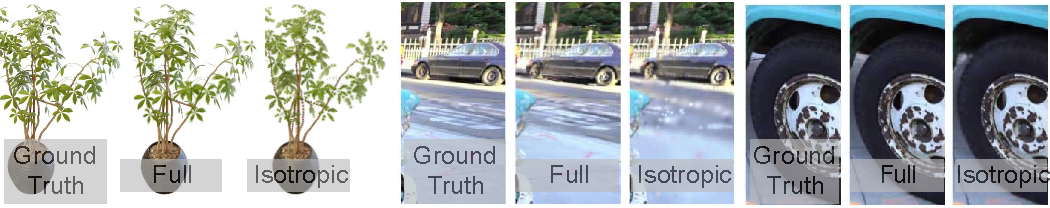
\includegraphics{figures/ablations/isotropy_vs_anisotropy2.pdf}
    \caption{
        \label{fig:ablation-aniso}
        Мы обучаем сцены с отключенной и включенной анизотропией Гауссиан. Использование анизотропных объемных сплатов позволяет моделировать мелкие структуры и оказывает значительное влияние на визуальное качество. Обратите внимание, что в иллюстративных целях мы ограничили \textsc{Ficus} использованием не более 5K Гауссиан в обеих конфигурациях.
    }
\end{figure*}

\paragraph{Сферические гармоники.}
Наконец, использование сферических гармоник улучшает наши общие показатели PSNR, поскольку они компенсируют зависимые от вида эффекты (\CORRECTION{Таб.}{Таблица}~\ref{tab:ablation_table}).

\subsection{Ограничения}
Наш метод не без ограничений.
В регионах, где сцена плохо наблюдаема, у нас есть артефакты; в таких регионах другие методы также сталкиваются с трудностями (например, Mip-NeRF360 на Рис.~\ref{fig:limit}). 
Хотя анизотропные Гауссианы имеют много преимуществ, как описано выше,
наш метод может создавать вытянутые артефакты или «пятнистые» Гауссианы (см. Рис.~\ref{fig:limit-under}); снова предыдущие методы также испытывают трудности в этих случаях.
У нас также иногда возникают скачкообразные артефакты, когда наша оптимизация создает большие Гауссианы; это обычно происходит в областях с зависимым от вида внешним видом.
Одной из причин этих скачкообразных артефактов является тривиальное отклонение Гауссиан через защитную полосу в растеризаторе. Более принципиальный подход к отбраковке мог бы уменьшить эти артефакты. \ADDITION{Другим фактором является наш простой алгоритм видимости, который может приводить к тому, что Гауссианы внезапно меняют порядок глубины/смешивания. Этого можно было бы избежать с помощью сглаживания, что мы оставляем для будущей работы.}
Кроме того, в настоящее время мы не применяем никакой регуляризации к нашей оптимизации; это помогло бы как с невидимыми областями, так и с скачкообразными артефактами.
\ADDITION{Хотя мы использовали одни и те же гиперпараметры для всей оценки, ранние эксперименты показывают, что уменьшение скорости обучения положения может быть необходимо для сходимости в очень больших сценах (например, городских наборах данных).}
Хотя мы весьма компактны по сравнению с предыдущими точечными подходами, потребление нашей памяти значительно выше, чем у решений на основе NeRF. \ADDITION{Во время обучения больших сцен пиковое потребление GPU-памяти может превышать 20 ГБ в нашей неоптимизированной прототипе. Однако эта цифра могла бы быть значительно снижена за счет тщательной низкоуровневой реализации логики оптимизации (аналогично InstantNGP). Рендеринг обученной сцены требует достаточного объема GPU-памяти для хранения полной модели (несколько сотен мегабайт для крупных сцен) и дополнительных 30--500 МБ для растеризатора, в зависимости от размера сцены и разрешения изображения. Мы отмечаем, что есть множество возможностей для дальнейшего снижения потребления памяти нашим методом.} Техники сжатия для облаков точек — это хорошо изученная область~\cite{de2016compression}; было бы интересно увидеть, как такие подходы могут быть адаптированы к нашему представлению.

\begin{figure}[!h]
    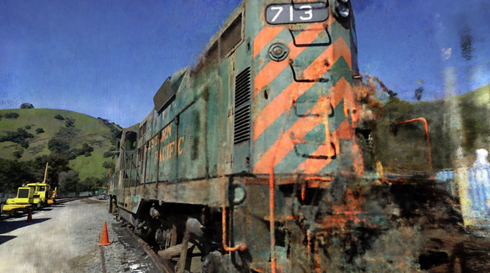
\includegraphics[width=0.49\columnwidth]{results/limitations/color_009_s.png}
    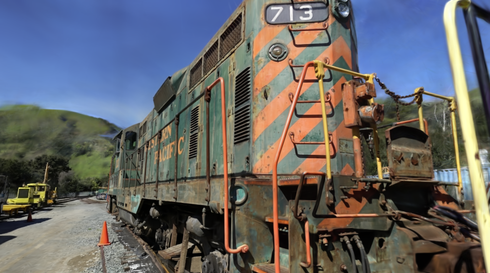
\includegraphics[width=0.49\columnwidth]{results/limitations/00073_s.png}
    \caption{
        \label{fig:limit}
        Сравнение артефактов сбоя: Mip-NeRF360 имеет «плавающие объекты» и зернистую текстуру (слева, передний план), тогда как наш метод производит грубые, анизотропные Гауссианы, приводящие к низкой детализации (справа, задний план). Сцена \textsc{Train}.
    }
\end{figure}

\begin{figure}[!h]
    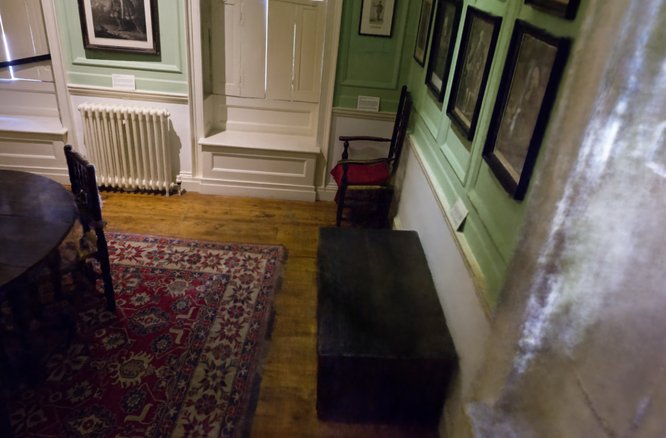
\includegraphics[width=0.49\linewidth]{figures/extremeviews/color_032_s.png}
    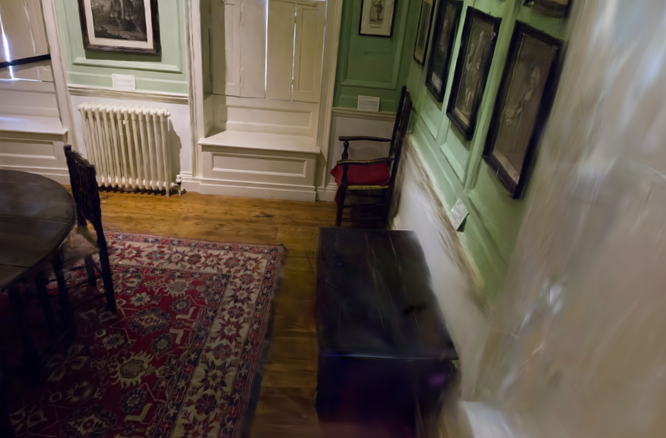
\includegraphics[width=0.49\linewidth]{figures/extremeviews/IMG_6589_s.png}
    \caption{
        В видах, которые мало пересекаются с теми, что были видны во время обучения, наш метод может производить артефакты (справа). Опять же, Mip-NeRF360 также имеет артефакты в этих случаях (слева). Сцена \textsc{DrJohnson}.
        \label{fig:limit-under}
    }
\end{figure}